\subsection{Arsitektur Dasar Acuan}

Arsitektur ini akan menjadi dasar acuan yang digunakan sebagai dasar perbandingan kinerja. Komponen \textit{backend} utama (layanan tiket) bersifat \textit{stateless}, sehingga dapat di-\textit{scale} dengan meningkatkan jumlah \textit{instance}. Kemudian, gerbang API akan melakukan \textit{load balancing} untuk mendistribusikan beban ke beberapa \textit{instance}.

\begin{figure}[htbp]
    \centering
    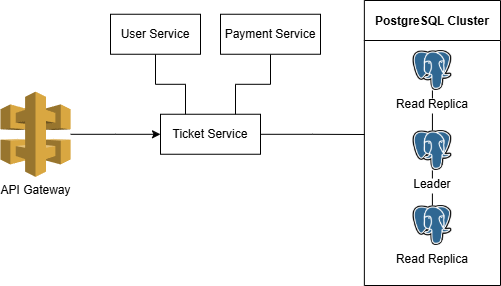
\includegraphics[width=0.8\textwidth]{resources/appendix/architecture-reference.png}
    \caption{Arsitektur Dasar Acuan}
    \label{fig:baseline-architecture}
\end{figure}

Basis data merupakan komponen yang sulit di-\textit{scale} secara dinamis berdasarkan beban yang diterima. Biasanya, penskalaan secara vertikal merupakan opsi utama untuk meningkatkan \textit{throughput}, terutama dalam operasi tulis. Meskipun begitu, pada arsitektur ini terdapat kluster PostgreSQL dengan konfigurasi satu node pemimpin dan sisanya node replika. Keberadaan replika memungkinkan peningkatan \textit{throughput} permintaan baca, meski tidak ada peningkatan \textit{throughput} untuk operasi tulis.